% id: 0230
% book: RPM 중3-2 수학 · 02 삼각비의 활용
% section: 중단원 마무리하기
% figure: crop:fig-0230.png
% answer: ③
% answer_source: 답지
% variant_level: 0 (원본 전사)
% 이 파일은 build.mjs 가 items.json 에서 만든다. 고칠 때는 items.json 을 고친다.
\noindent\begin{minipage}[t]{0.58\linewidth}\vspace{0pt}\raggedright 오른쪽 그림과 같은 평행사변형~$\pt{ABCD}$에서 대각선~$\pt{BD}$의 길이는?\end{minipage}\hfill\begin{minipage}[t]{0.4\linewidth}\vspace{0pt}\centering \setlength{\dmfigw}{103.7pt}\ifdim\dmfigw>\linewidth\setlength{\dmfigw}{\linewidth}\fi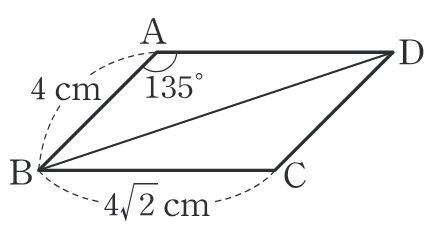
\includegraphics[width=\dmfigw]{figures/fig-0230.png}\end{minipage}\par
\begin{choicesii}{\rule[-3ex]{0pt}{8ex}$8\mkern3mu \mathrm{cm}$}{\rule[-3ex]{0pt}{8ex}$6\sqrt{2}\mkern3mu \mathrm{cm}$}{\rule[-3ex]{0pt}{8ex}$4\sqrt{5}\mkern3mu \mathrm{cm}$}{\rule[-3ex]{0pt}{8ex}$3\sqrt{10}\mkern3mu \mathrm{cm}$}{\rule[-3ex]{0pt}{8ex}$4\sqrt{6}\mkern3mu \mathrm{cm}$}\end{choicesii}
